%Version 3.1 December 2024
% See section 11 of the User Manual for version history
%
%%%%%%%%%%%%%%%%%%%%%%%%%%%%%%%%%%%%%%%%%%%%%%%%%%%%%%%%%%%%%%%%%%%%%%
%%                                                                 %%
%% Please do not use \input{...} to include other tex files.       %%
%% Submit your LaTeX manuscript as one .tex document.              %%
%%                                                                 %%
%% All additional figures and files should be attached             %%
%% separately and not embedded in the \TeX\ document itself.       %%
%%                                                                 %%
%%%%%%%%%%%%%%%%%%%%%%%%%%%%%%%%%%%%%%%%%%%%%%%%%%%%%%%%%%%%%%%%%%%%%

%%\documentclass[referee,sn-basic]{sn-jnl}% referee option is meant for double line spacing

%%=======================================================%%
%% to print line numbers in the margin use lineno option %%
%%=======================================================%%

%%\documentclass[lineno,pdflatex,sn-basic]{sn-jnl}% Basic Springer Nature Reference Style/Chemistry Reference Style

%%=========================================================================================%%
%% the documentclass is set to pdflatex as default. You can delete it if not appropriate.  %%
%%=========================================================================================%%

%%\documentclass[sn-basic]{sn-jnl}% Basic Springer Nature Reference Style/Chemistry Reference Style

%%Note: the following reference styles support Namedate and Numbered referencing. By default the style follows the most common style. To switch between the options you can add or remove “Numbered” in the optional parenthesis. 
%%The option is available for: sn-basic.bst, sn-chicago.bst%  
 
%%\documentclass[pdflatex,sn-nature]{sn-jnl}% Style for submissions to Nature Portfolio journals
%%\documentclass[pdflatex,sn-basic]{sn-jnl}% Basic Springer Nature Reference Style/Chemistry Reference Style
\documentclass[pdflatex,sn-mathphys-num]{sn-jnl}% Math and Physical Sciences Numbered Reference Style
%%\documentclass[pdflatex,sn-mathphys-ay]{sn-jnl}% Math and Physical Sciences Author Year Reference Style
%%\documentclass[pdflatex,sn-aps]{sn-jnl}% American Physical Society (APS) Reference Style
%%\documentclass[pdflatex,sn-vancouver-num]{sn-jnl}% Vancouver Numbered Reference Style
%%\documentclass[pdflatex,sn-vancouver-ay]{sn-jnl}% Vancouver Author Year Reference Style
%%\documentclass[pdflatex,sn-apa]{sn-jnl}% APA Reference Style
%%\documentclass[pdflatex,sn-chicago]{sn-jnl}% Chicago-based Humanities Reference Style

%%%% Standard Packages
%%<additional latex packages if required can be included here>

\usepackage{graphicx}%
\usepackage{multirow}%
\usepackage{amsmath,amssymb,amsfonts}%
\usepackage{amsthm}%
\usepackage{mathrsfs}%
\usepackage[title]{appendix}%
\usepackage{xcolor}%
\usepackage{textcomp}%
\usepackage{manyfoot}%
\usepackage{booktabs}%
\usepackage{algorithm}%
\usepackage{algorithmicx}%
\usepackage{algpseudocode}%
\usepackage{listings}%

\usepackage{kotex}
%%%%

%%%%%=============================================================================%%%%
%%%%  Remarks: This template is provided to aid authors with the preparation
%%%%  of original research articles intended for submission to journals published 
%%%%  by Springer Nature. The guidance has been prepared in partnership with 
%%%%  production teams to conform to Springer Nature technical requirements. 
%%%%  Editorial and presentation requirements differ among journal portfolios and 
%%%%  research disciplines. You may find sections in this template are irrelevant 
%%%%  to your work and are empowered to omit any such section if allowed by the 
%%%%  journal you intend to submit to. The submission guidelines and policies 
%%%%  of the journal take precedence. A detailed User Manual is available in the 
%%%%  template package for technical guidance.
%%%%%=============================================================================%%%%

%% as per the requirement new theorem styles can be included as shown below
\theoremstyle{thmstyleone}%
\newtheorem{theorem}{Theorem}%  meant for continuous numbers
%%\newtheorem{theorem}{Theorem}[section]% meant for sectionwise numbers
%% optional argument [theorem] produces theorem numbering sequence instead of independent numbers for Proposition
\newtheorem{proposition}[theorem]{Proposition}% 
%%\newtheorem{proposition}{Proposition}% to get separate numbers for theorem and proposition etc.

\theoremstyle{thmstyletwo}%
\newtheorem{example}{Example}%
\newtheorem{remark}{Remark}%

\theoremstyle{thmstylethree}%
\newtheorem{definition}{Definition}%

\raggedbottom
%%\unnumbered% uncomment this for unnumbered level heads

\begin{document}

\title[Article Title]{User-Adjustable UI for Concurrent PDF and Whiteboard Display in Live Mobile Learning System}

%%=============================================================%%
%% GivenName	-> \fnm{Joergen W.}
%% Particle	-> \spfx{van der} -> surname prefix
%% FamilyName	-> \sur{Ploeg}
%% Suffix	-> \sfx{IV}
%% \author*[1,2]{\fnm{Joergen W.} \spfx{van der} \sur{Ploeg} 
%%  \sfx{IV}}\email{iauthor@gmail.com}
%%=============================================================%%

\author{\fnm{Hosung} \sur{Kim}}\email{hosungkim5108@gmail.com}

%%\author[2,3]{\fnm{Second} \sur{Author}}\email{iiauthor@gmail.com}
%%\equalcont{These authors contributed equally to this work.}

%%\author[1,2]{\fnm{Third} \sur{Author}}\email{iiiauthor@gmail.com}
%%\equalcont{These authors contributed equally to this work.}

\affil{\orgdiv{Department of Computer Engineering}, \orgname{Hongik University}, \orgaddress{ \city{Seoul}, \country{Korea}}}

\abstract{본 보고서는 강의자료와 화이트보드를 동시에 시각적으로 제공하지 못하는 기존 모바일 원격 교육 시스템의 한계를 해결하기 위해, User-Adjustable UI를 설계하고 구현한 내용을 다룬다. 제안된 UI는 grabber를 통해 강의자가 두 콘텐츠 영역의 크기를 실시간으로 조절할 수 있도록 하여 실제 강의 환경과 유사한 병렬적 정보 제공을 가능하게 한다. 또한 참여자 목록과 채팅창 접이식 구조로 개선하여 불필요한 화면 점유를 줄였다. 이를 통해 제한된 화면 공간을 보다 효율적으로 활용하여 학습 경험의 질을 향상시킬 수 있다. (향후 과제는 교수님 피드백을 반영하여 추후 작성 예정)}

%%\keywords{keyword1, Keyword2, Keyword3, Keyword4}

%%\pacs[JEL Classification]{D8, H51}

%%\pacs[MSC Classification]{35A01, 65L10, 65L12, 65L20, 65L70}

\maketitle

\section{Introduction}\label{sec1}

선행 보고서에서는 기존의 모바일 원격 교육 시스템을 다중 강의실 구조로 확장하고, 강의자 카메라 프리뷰, 화이트보드, 참여자 현황 표시 등 다양한 기능을 추가하여 실시간 상호작용성을 향상시켰다. 특히 PDF 강의자료와 화이트보드 기능의 경우, 제한된 화면 공간에서 UI 요소의 크기가 지나치게 작아지는 문제를 방지하기 위해, \verb+UISegmentedControl+을 사용한 전환 방식으로 강의자료와 공유 화이트보드 중 하나를 선택적으로 표시하는 방식을 적용하였다. 그러나 이 방식은 강의자료와 칠판이 병렬적으로 제공되는 실제 강의 환경의 특성을 반영하지 못한다는 한계가 있었다. 이에 본 보고서에서는 강의자료와 화이트보드를 동시에 제공하면서도 제한된 화면 공간을 효율적으로 활용할 수 있는 User-Adjustable UI를 설계 및 구현하였다.

\section{User-Adjustable UI for Concurrent PDF and Whiteboard Display}\label{sec2}

\begin{figure}[p]
\centering
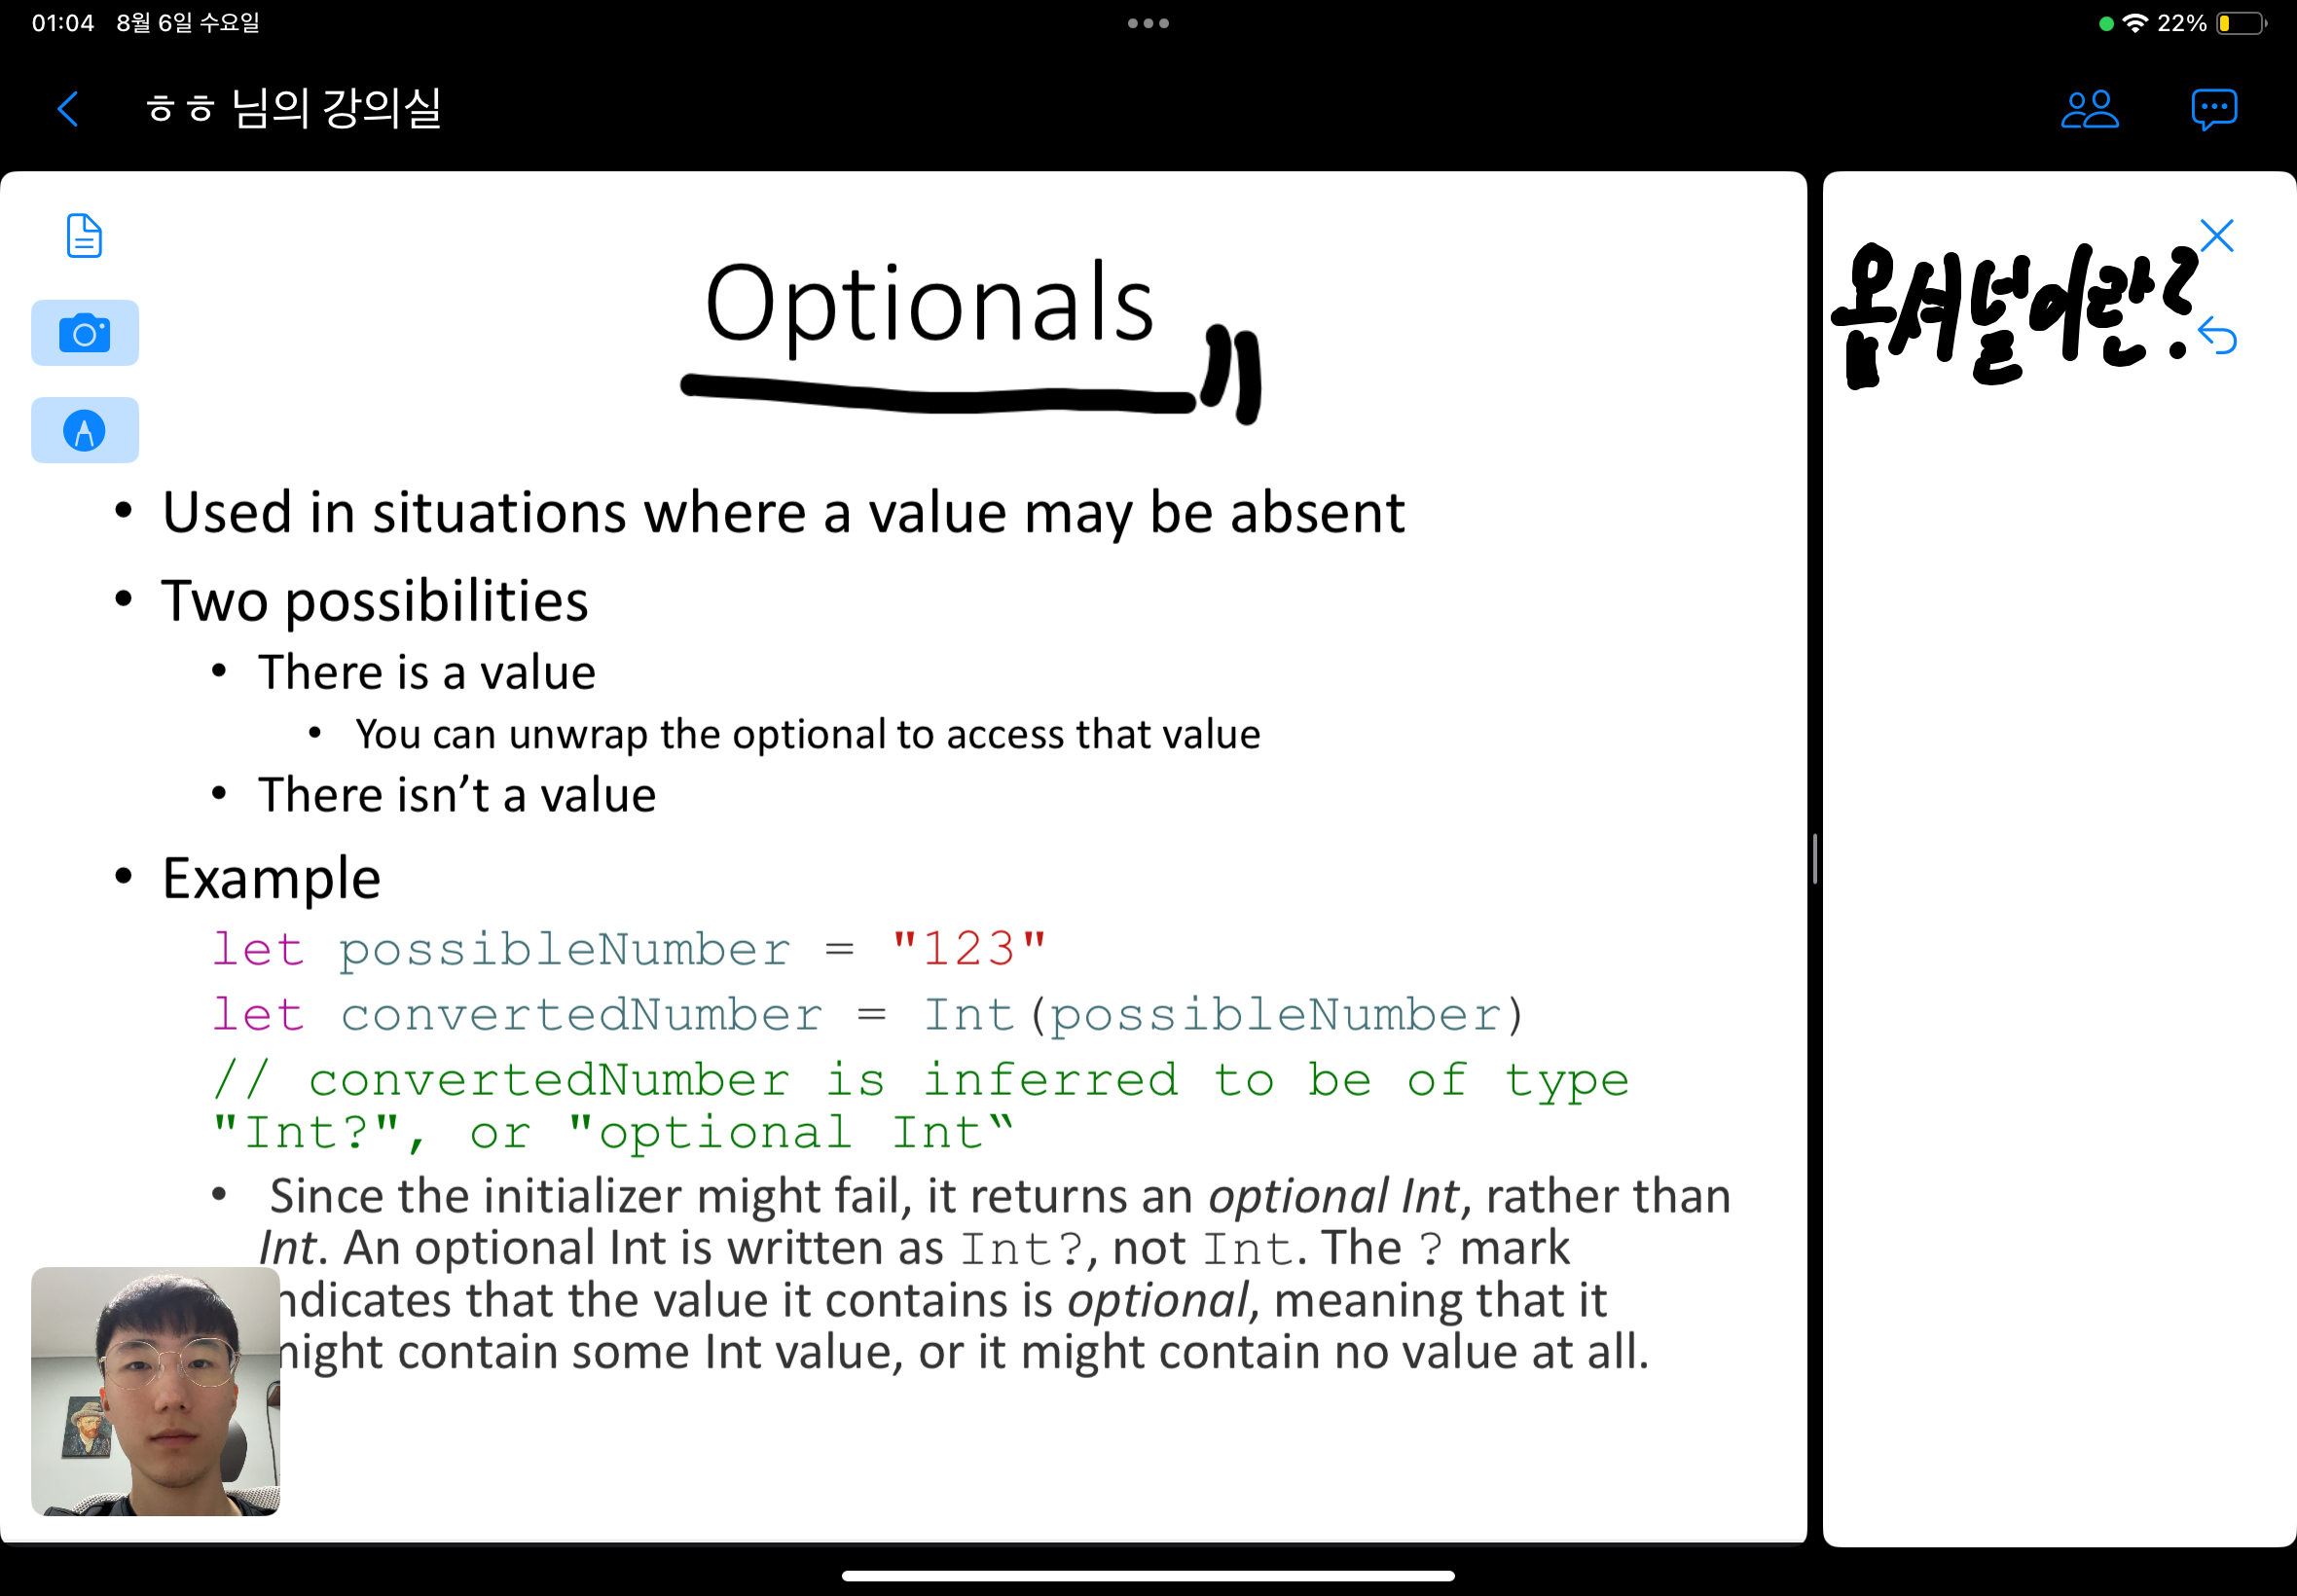
\includegraphics[width=0.9\textwidth]{UserInterfaceWithAnExpandedDocumentArea.PNG}
\caption{User interface with an expanded document area}\label{fig1}
\end{figure}

\begin{figure}[p]
\centering
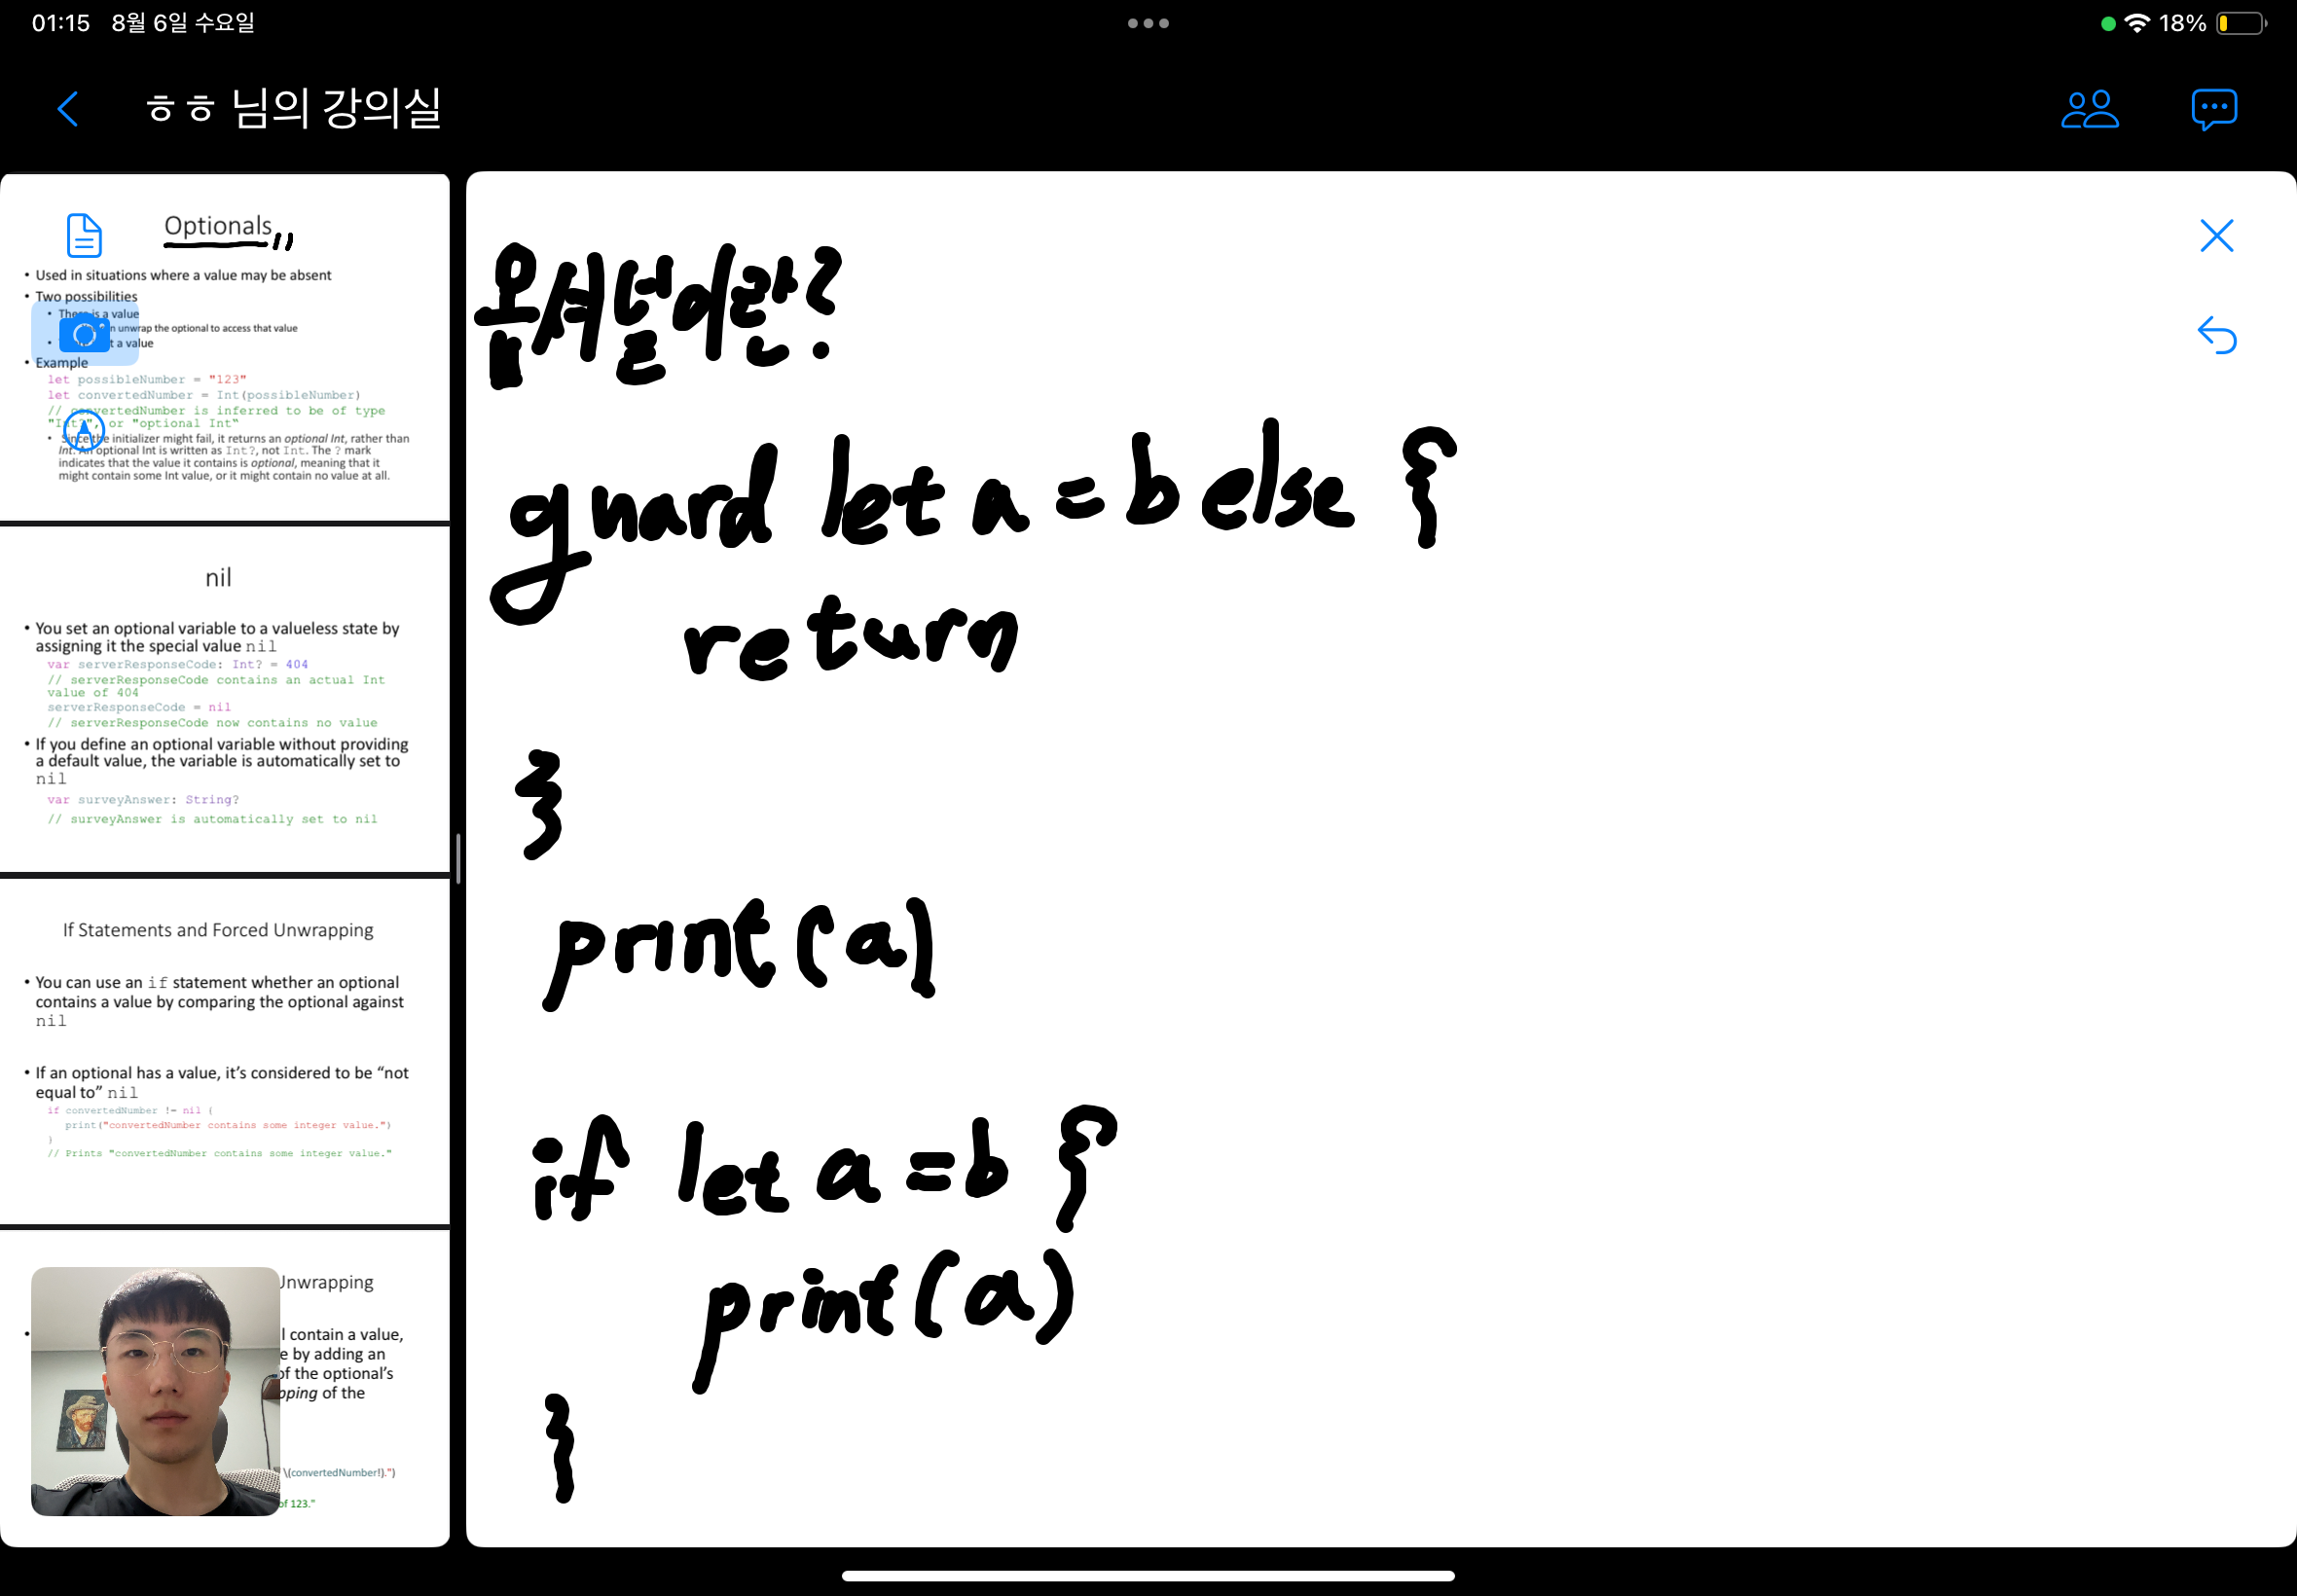
\includegraphics[width=0.9\textwidth]{UserInterfaceWithAnExpandedWhiteboardArea.PNG}
\caption{User interface with an expanded whiteboard area}\label{fig2}
\end{figure}

강의자료와 화이트보드가 지나치게 작다면 강의자가 이를 효과적으로 활용하기 어렵고 학생의 이해도 역시 저하될 수 있다. 본 시스템은 이러한 문제를 해결하기 위해 강의자가 강의자료와 화이트보드 두 콘텐츠 영역의 크기를 조절할 수 있는 User-Adjustable UI를 제안한다. 강의자는 grabber를 드래그하여 강의자료와 화이트보드의 화면 비율을 자유롭게 조절하며 강의 상황에 따라 필요한 정보를 유연하게 강조할 수 있다.

grabber는 \verb+UISlider+\cite{UISlider}를 기반으로 구현되었으며, 사용자의 조작으로 value가 변경되면 \verb+valueChanged+ 이벤트를 통해 강의자료와 공유 화이트보드 화면 비율을 결정하는 \verb+NSLayoutConstraint+의 \verb+multiplier+값에 해당 값을 반영하였다. \verb+UISlider+는 clear color로 설정하여 로직적인 역할만을 수행하도록 화면에 드러나지 않게 하였다.

또한 채팅창과 참여자 목록은 접이식 구조로 재구성하여 필요할 때만 표시되도록 하였다. 두 구성요소는 \verb+UIStackView+에 포함되어 있으며, 우측 상단 각각의 토글 버튼에 따라 \verb+isHidden+ 속성을 조정함으로써 열고 닫을 수 있다. 이를 통해 불필요한 화면 점유를 최소화하였다.

이 외에도 참여자 목록과 채팅창 이름 옆에 강사 혹은 본인임을 식별할 수 있는 \verb+Label+을 추가하는 등 소규모 UI 개선도 함께 이루어졌다.

\section{Conclusion}\label{sec3}

본 보고서에서는 강의자료와 화이트보드를 동시에 시각적으로 제공하지 못하는 기존 시스템의 한계를 해결하기 위해 User-Adjustable UI를 설계 및 구현하였다. 제안된 UI는 \verb+UISlider+ 기반의 grabber를 통해 강의자가 두 콘텐츠 영역의 비율을 실시간으로 조절할 수 있도록 하여 실제 강의 환경과 유사한 병렬적 정보 제공을 효과적으로 지원한다.

또한 참여자 목록과 채팅창은 접이식 구조로 재구성되어 불필요한 화면 점유를 최소화함으로써 제한된 화면 공간의 활용도를 높이고 학습 콘텐츠에 대한 시각적 집중을 강화하였다.

(향후 과제는 교수님 피드백을 반영하여 추후 작성 예정)

전체 소스코드는 \href{https://github.com/H0sungKim/CollaborativeComputingLab}{https://github.com/H0sungKim/CollaborativeComputingLab}에서 확인할 수 있다.

%===========================================================================================%%
%% If you are submitting to one of the Nature Portfolio journals, using the eJP submission   %%
%% system, please include the references within the manuscript file itself. You may do this  %%
%% by copying the reference list from your .bbl file, paste it into the main manuscript .tex %%
%% file, and delete the associated \verb+\bibliography+ commands.                            %%
%%===========================================================================================%%

\bibliography{bibliography}

\end{document}
